% Options for packages loaded elsewhere
\PassOptionsToPackage{unicode}{hyperref}
\PassOptionsToPackage{hyphens}{url}
%
\documentclass[
  10pt,a4paper,
]{article}
\usepackage{amsmath,amssymb}
\usepackage{iftex}
\ifPDFTeX
  \usepackage[T1]{fontenc}
  \usepackage[utf8]{inputenc}
  \usepackage{textcomp} % provide euro and other symbols
\else % if luatex or xetex
  \usepackage{unicode-math} % this also loads fontspec
  \defaultfontfeatures{Scale=MatchLowercase}
  \defaultfontfeatures[\rmfamily]{Ligatures=TeX,Scale=1}
\fi
\usepackage{lmodern}
\ifPDFTeX\else
  % xetex/luatex font selection
\fi
% Use upquote if available, for straight quotes in verbatim environments
\IfFileExists{upquote.sty}{\usepackage{upquote}}{}
\IfFileExists{microtype.sty}{% use microtype if available
  \usepackage[]{microtype}
  \UseMicrotypeSet[protrusion]{basicmath} % disable protrusion for tt fonts
}{}
\makeatletter
\@ifundefined{KOMAClassName}{% if non-KOMA class
  \IfFileExists{parskip.sty}{%
    \usepackage{parskip}
  }{% else
    \setlength{\parindent}{0pt}
    \setlength{\parskip}{6pt plus 2pt minus 1pt}}
}{% if KOMA class
  \KOMAoptions{parskip=half}}
\makeatother
\usepackage{xcolor}
\usepackage[margin=20mm]{geometry}
\usepackage{longtable,booktabs,array}
\usepackage{calc} % for calculating minipage widths
% Correct order of tables after \paragraph or \subparagraph
\usepackage{etoolbox}
\makeatletter
\patchcmd\longtable{\par}{\if@noskipsec\mbox{}\fi\par}{}{}
\makeatother
% Allow footnotes in longtable head/foot
\IfFileExists{footnotehyper.sty}{\usepackage{footnotehyper}}{\usepackage{footnote}}
\makesavenoteenv{longtable}
\usepackage{graphicx}
\makeatletter
\def\maxwidth{\ifdim\Gin@nat@width>\linewidth\linewidth\else\Gin@nat@width\fi}
\def\maxheight{\ifdim\Gin@nat@height>\textheight\textheight\else\Gin@nat@height\fi}
\makeatother
% Scale images if necessary, so that they will not overflow the page
% margins by default, and it is still possible to overwrite the defaults
% using explicit options in \includegraphics[width, height, ...]{}
\setkeys{Gin}{width=\maxwidth,height=\maxheight,keepaspectratio}
% Set default figure placement to htbp
\makeatletter
\def\fps@figure{htbp}
\makeatother
\setlength{\emergencystretch}{3em} % prevent overfull lines
\providecommand{\tightlist}{%
  \setlength{\itemsep}{0pt}\setlength{\parskip}{0pt}}
\setcounter{secnumdepth}{-\maxdimen} % remove section numbering
\ifLuaTeX
  \usepackage{selnolig}  % disable illegal ligatures
\fi
\usepackage{bookmark}
\IfFileExists{xurl.sty}{\usepackage{xurl}}{} % add URL line breaks if available
\urlstyle{same}
\hypersetup{
  hidelinks,
  pdfcreator={LaTeX via pandoc}}

\author{}
\date{}

\begin{document}

\emph{Network-triggered cultural ignition as a candidate Great Filter}

Mykola Shatokhin

\section{S1. Model parameters and
diagnostics}\label{s1.-model-parameters-and-diagnostics}

The model consists of agents nested in groups, six cultural domains and
five prerequisite levels. Reproduction samples parents according to
repertoire benefit and cognitive cost. Learners observe local or
external models, copy prerequisite chains with level-dependent error,
recombine the best domain levels from multiple models and innovate.
Teaching, adaptive model number and infrastructure are continuous
functions of observed repertoires, not binary switches. Table S1 lists
the reference configuration; Figures S1 and S2 report global parameter
sensitivity and outcome-definition robustness.

Table S1. Reference model configuration and outcome diagnostics.

\begin{longtable}[]{@{}
  >{\raggedright\arraybackslash}p{(\columnwidth - 2\tabcolsep) * \real{0.4865}}
  >{\raggedright\arraybackslash}p{(\columnwidth - 2\tabcolsep) * \real{0.4865}}@{}}
\toprule\noalign{}
\begin{minipage}[b]{\linewidth}\raggedright
Quantity
\end{minipage} & \begin{minipage}[b]{\linewidth}\raggedright
Reference value
\end{minipage} \\
\midrule\noalign{}
\endhead
\bottomrule\noalign{}
\endlastfoot
Groups x agents & 16 x 20 \\
Domains x levels & 6 x 5 \\
Generations & 420 \\
Years per generation & 25 \\
Baseline external-model probability & 0.002 \\
Primary individual diagnostic & S \textgreater= 16 and \textgreater=5
developed domains \\
Persistent population diagnostic & \textgreater50\% agents for 45/50
final generations; mean S \textgreater18 \\
\end{longtable}

\begin{figure}
\centering
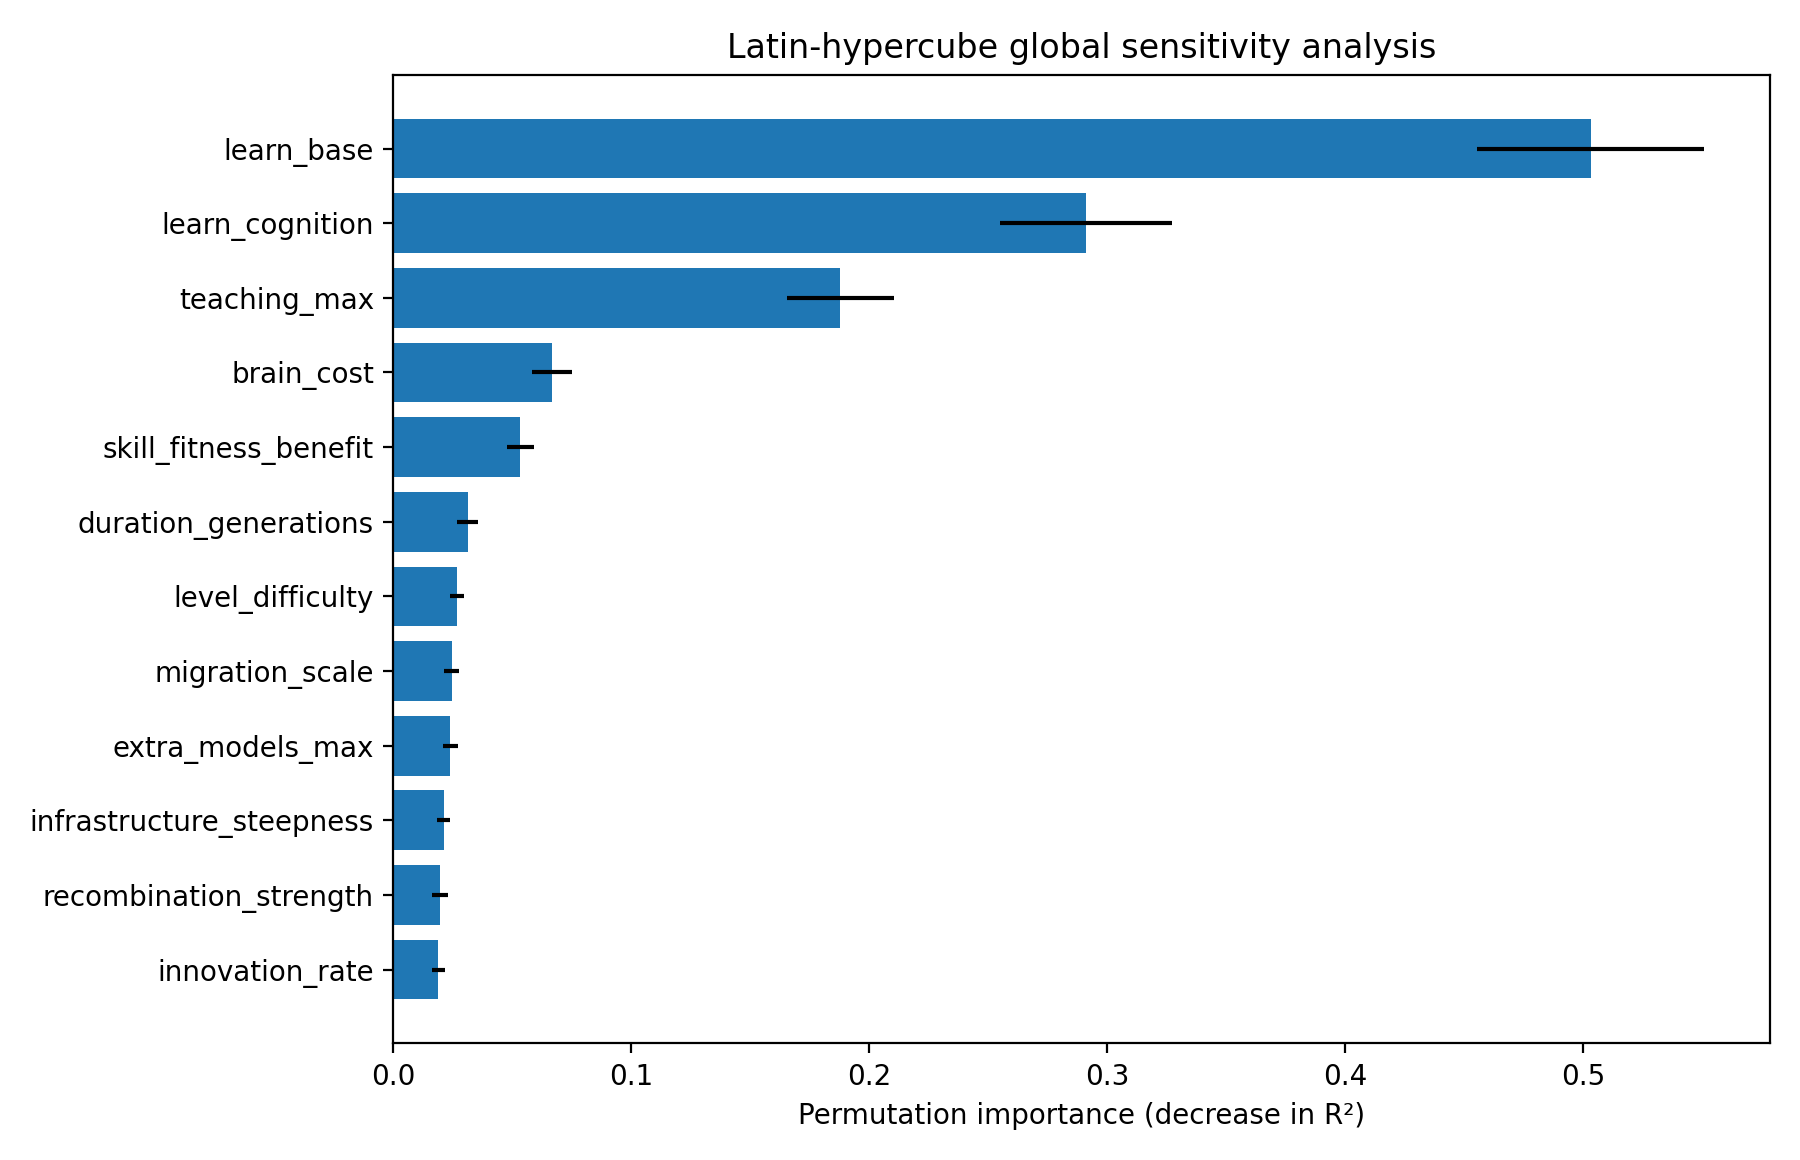
\includegraphics[width=6.2in,height=3.99556in]{figS1.png}
\caption{Bar plot of permutation importance and associations for
fourteen model parameters.}
\end{figure}

Figure S1. Global Latin-hypercube sensitivity analysis.

\begin{figure}
\centering
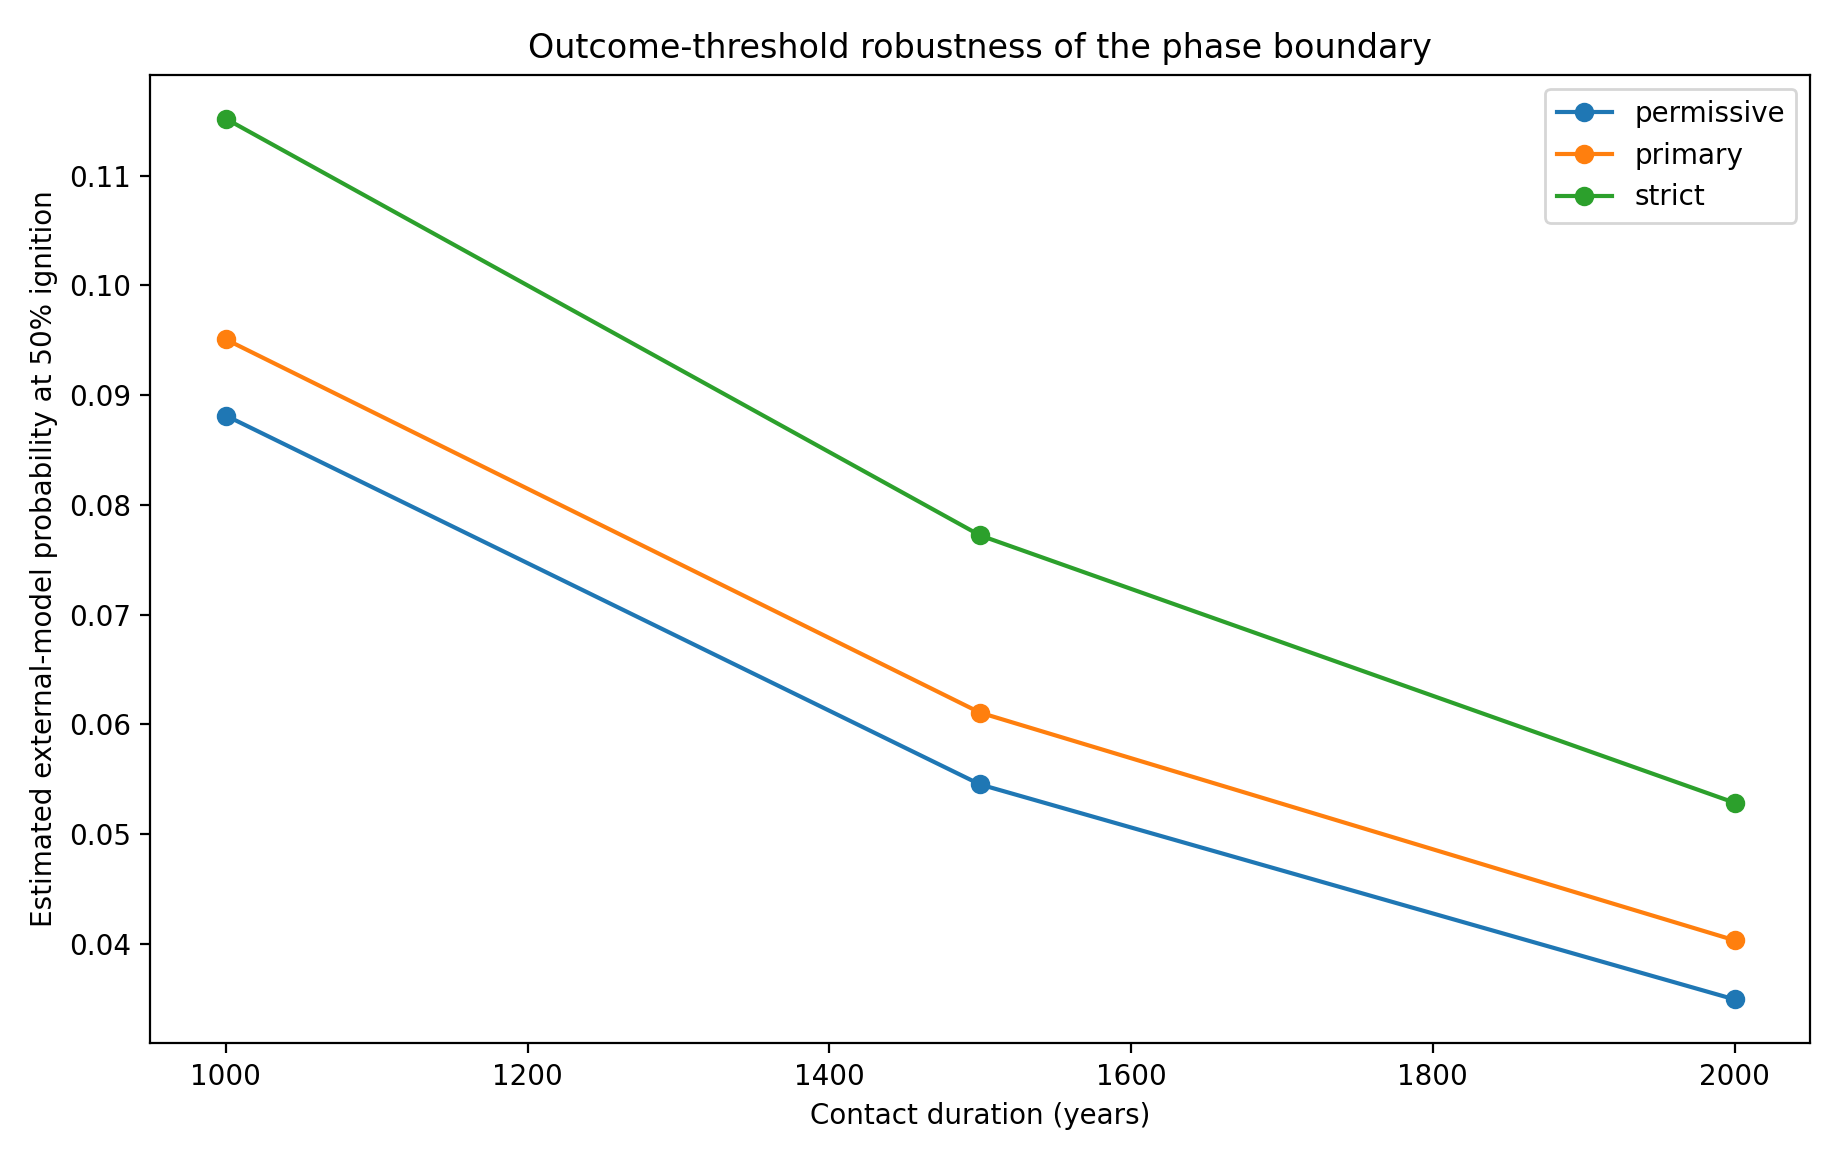
\includegraphics[width=6.2in,height=3.91082in]{figS2.png}
\caption{Curves compare the estimated phase boundary under three outcome
definitions.}
\end{figure}

Figure S2. Ignition boundaries under permissive, primary and strict
diagnostics.

\section{S2. Expanded ablation
results}\label{s2.-expanded-ablation-results}

Table S2 reports duration-specific boundaries for the full model and
each ablation in the expanded grid. This grid uses four contact values and
50 replicates per cell, whereas the primary dense phase experiment uses nine
contact values and 100 replicates per cell. The full-model values in Table S2
are therefore separate robustness estimates, not replacements for the dense
phase thresholds reported in the main text.

Table S2. Expanded ablation boundaries across contact duration.

\begin{longtable}[]{@{}
  >{\raggedright\arraybackslash}p{(\columnwidth - 6\tabcolsep) * \real{0.2432}}
  >{\raggedright\arraybackslash}p{(\columnwidth - 6\tabcolsep) * \real{0.2432}}
  >{\raggedright\arraybackslash}p{(\columnwidth - 6\tabcolsep) * \real{0.2432}}
  >{\raggedright\arraybackslash}p{(\columnwidth - 6\tabcolsep) * \real{0.2432}}@{}}
\toprule\noalign{}
\begin{minipage}[b]{\linewidth}\raggedright
Model
\end{minipage} & \begin{minipage}[b]{\linewidth}\raggedright
Duration (years)
\end{minipage} & \begin{minipage}[b]{\linewidth}\raggedright
Estimated p50
\end{minipage} & \begin{minipage}[b]{\linewidth}\raggedright
Maximum observed P
\end{minipage} \\
\midrule\noalign{}
\endhead
\bottomrule\noalign{}
\endlastfoot
Full model & 1000 & 0.107 & 0.72 \\
Full model & 1500 & 0.064 & 0.88 \\
Full model & 2000 & 0.041 & 0.94 \\
No cultural selection on cognition & 1000 & 1.124 & 0.02 \\
No cultural selection on cognition & 1500 & 0.217 & 0.18 \\
No cultural selection on cognition & 2000 & 0.193 & 0.26 \\
No infrastructure feedback & 1000 & not reached & 0.00 \\
No infrastructure feedback & 1500 & not reached & 0.00 \\
No infrastructure feedback & 2000 & not reached & 0.00 \\
No recombination & 1000 & not reached & 0.00 \\
No recombination & 1500 & not reached & 0.00 \\
No recombination & 2000 & not reached & 0.00 \\
No teaching & 1000 & not reached & 0.00 \\
No teaching & 1500 & not reached & 0.00 \\
No teaching & 2000 & not reached & 0.00 \\
\end{longtable}

Zero ignition in the tested grid establishes component dependence only for
$p_{\rm ext}\leq 0.16$, contact duration $\leq 2000$ years and
the remaining reference parameters of this model architecture. It does not
establish universal biological necessity and does not preclude ignition under
untested extremes or alternative mechanisms.

\section{S3. Archaeological
robustness}\label{s3.-archaeological-robustness}

Table S3 summarizes date and cluster uncertainty. Figures S3 and S4 show
the permutation null and threshold sensitivity; Table S4 gives the
fixed-boundary results.

Table S3. Archaeological change-point estimates under date and cluster
uncertainty.

\begin{longtable}[]{@{}
  >{\raggedright\arraybackslash}p{(\columnwidth - 4\tabcolsep) * \real{0.3243}}
  >{\raggedright\arraybackslash}p{(\columnwidth - 4\tabcolsep) * \real{0.3243}}
  >{\raggedright\arraybackslash}p{(\columnwidth - 4\tabcolsep) * \real{0.3243}}@{}}
\toprule\noalign{}
\begin{minipage}[b]{\linewidth}\raggedright
Analysis
\end{minipage} & \begin{minipage}[b]{\linewidth}\raggedright
Median change point
\end{minipage} & \begin{minipage}[b]{\linewidth}\raggedright
95\% interval
\end{minipage} \\
\midrule\noalign{}
\endhead
\bottomrule\noalign{}
\endlastfoot
Midpoint optimum & 525 ka & - \\
Dates sampled in intervals & 500 ka & 325-575 ka \\
Source-cluster bootstrap & 525 ka & 275-575 ka \\
Site-cluster bootstrap & 525 ka & 275-575 ka \\
\end{longtable}

\begin{figure}
\centering
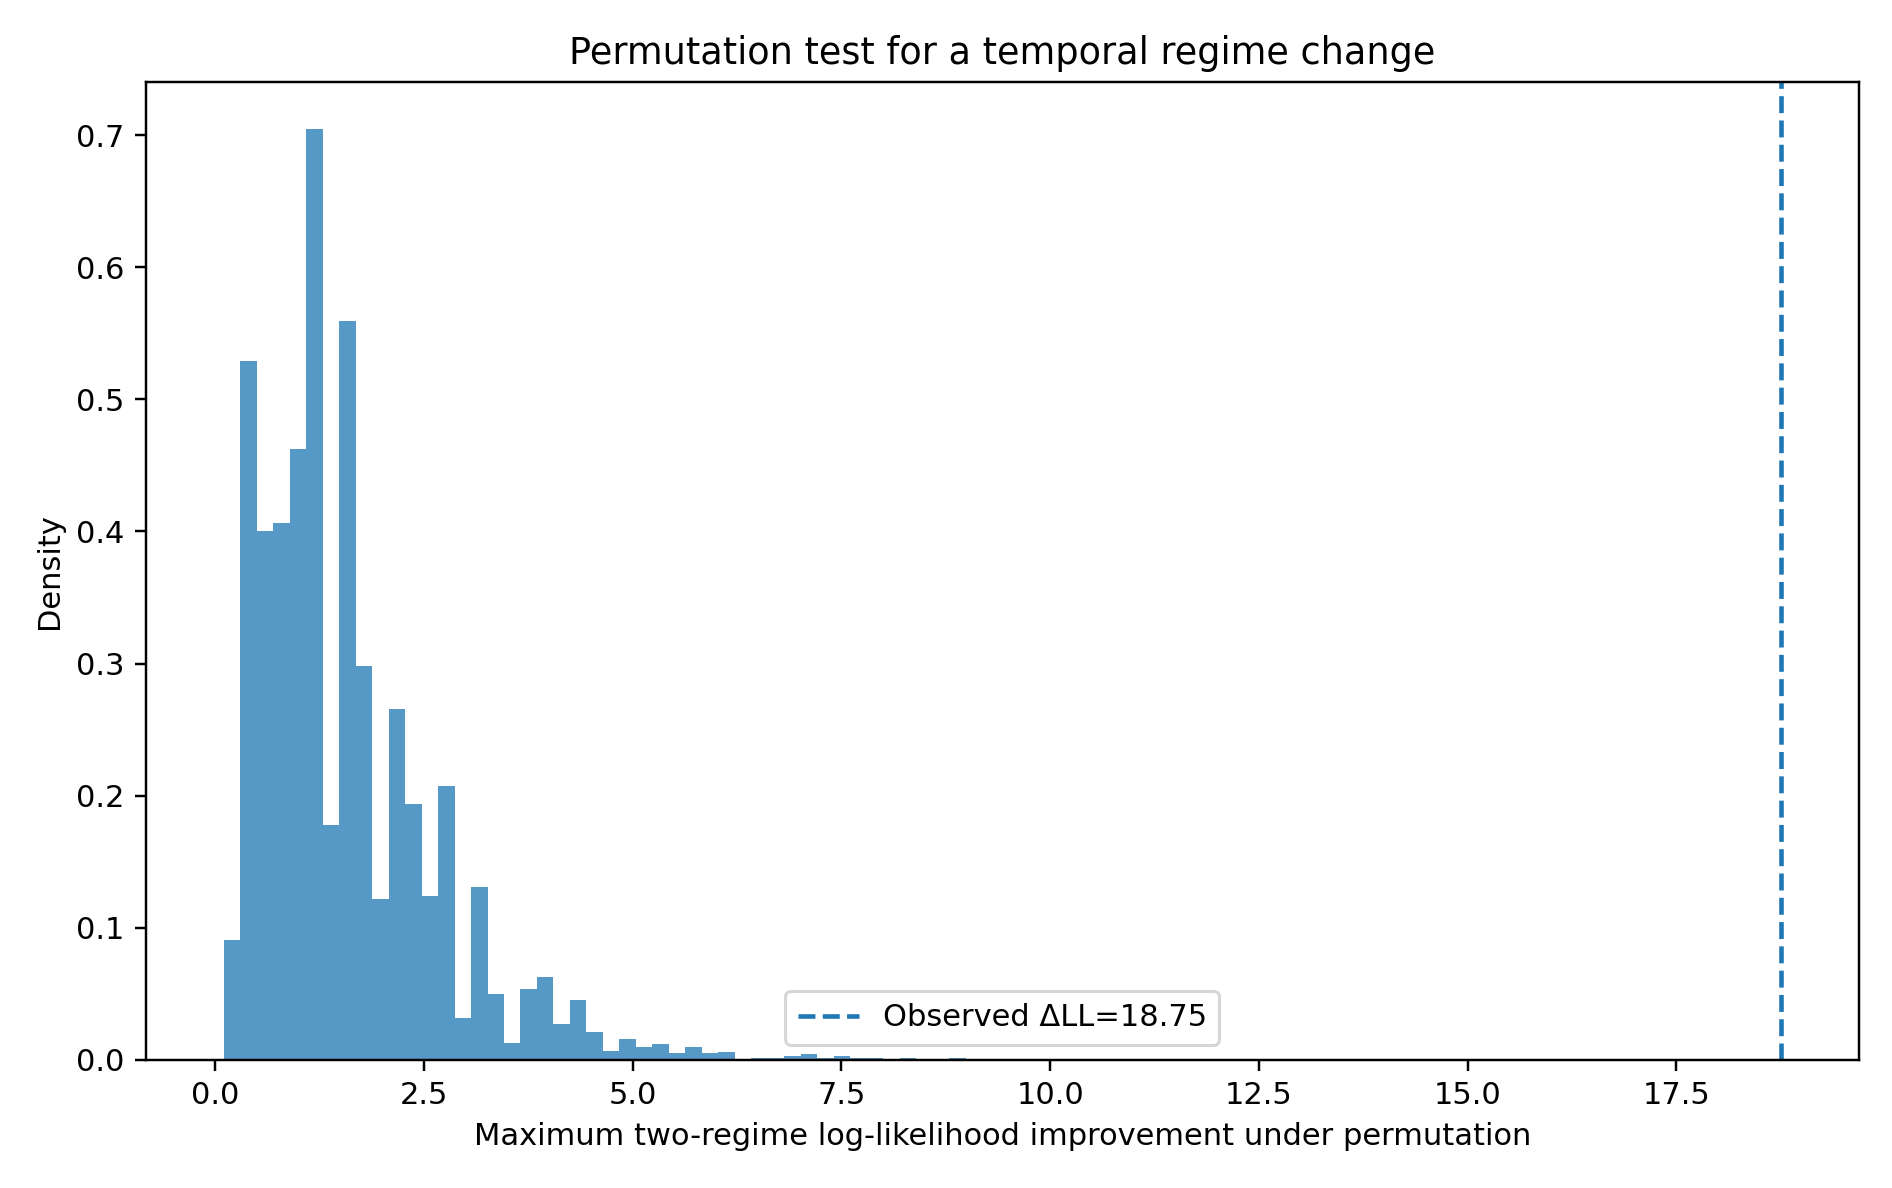
\includegraphics[width=6in,height=3.76744in]{figS3.png}
\caption{Histogram of permutation delta log-likelihood values with the
observed value marked beyond the distribution.}
\end{figure}

Figure S3. Temporal permutation test for the archaeological change
point.

\begin{figure}
\centering
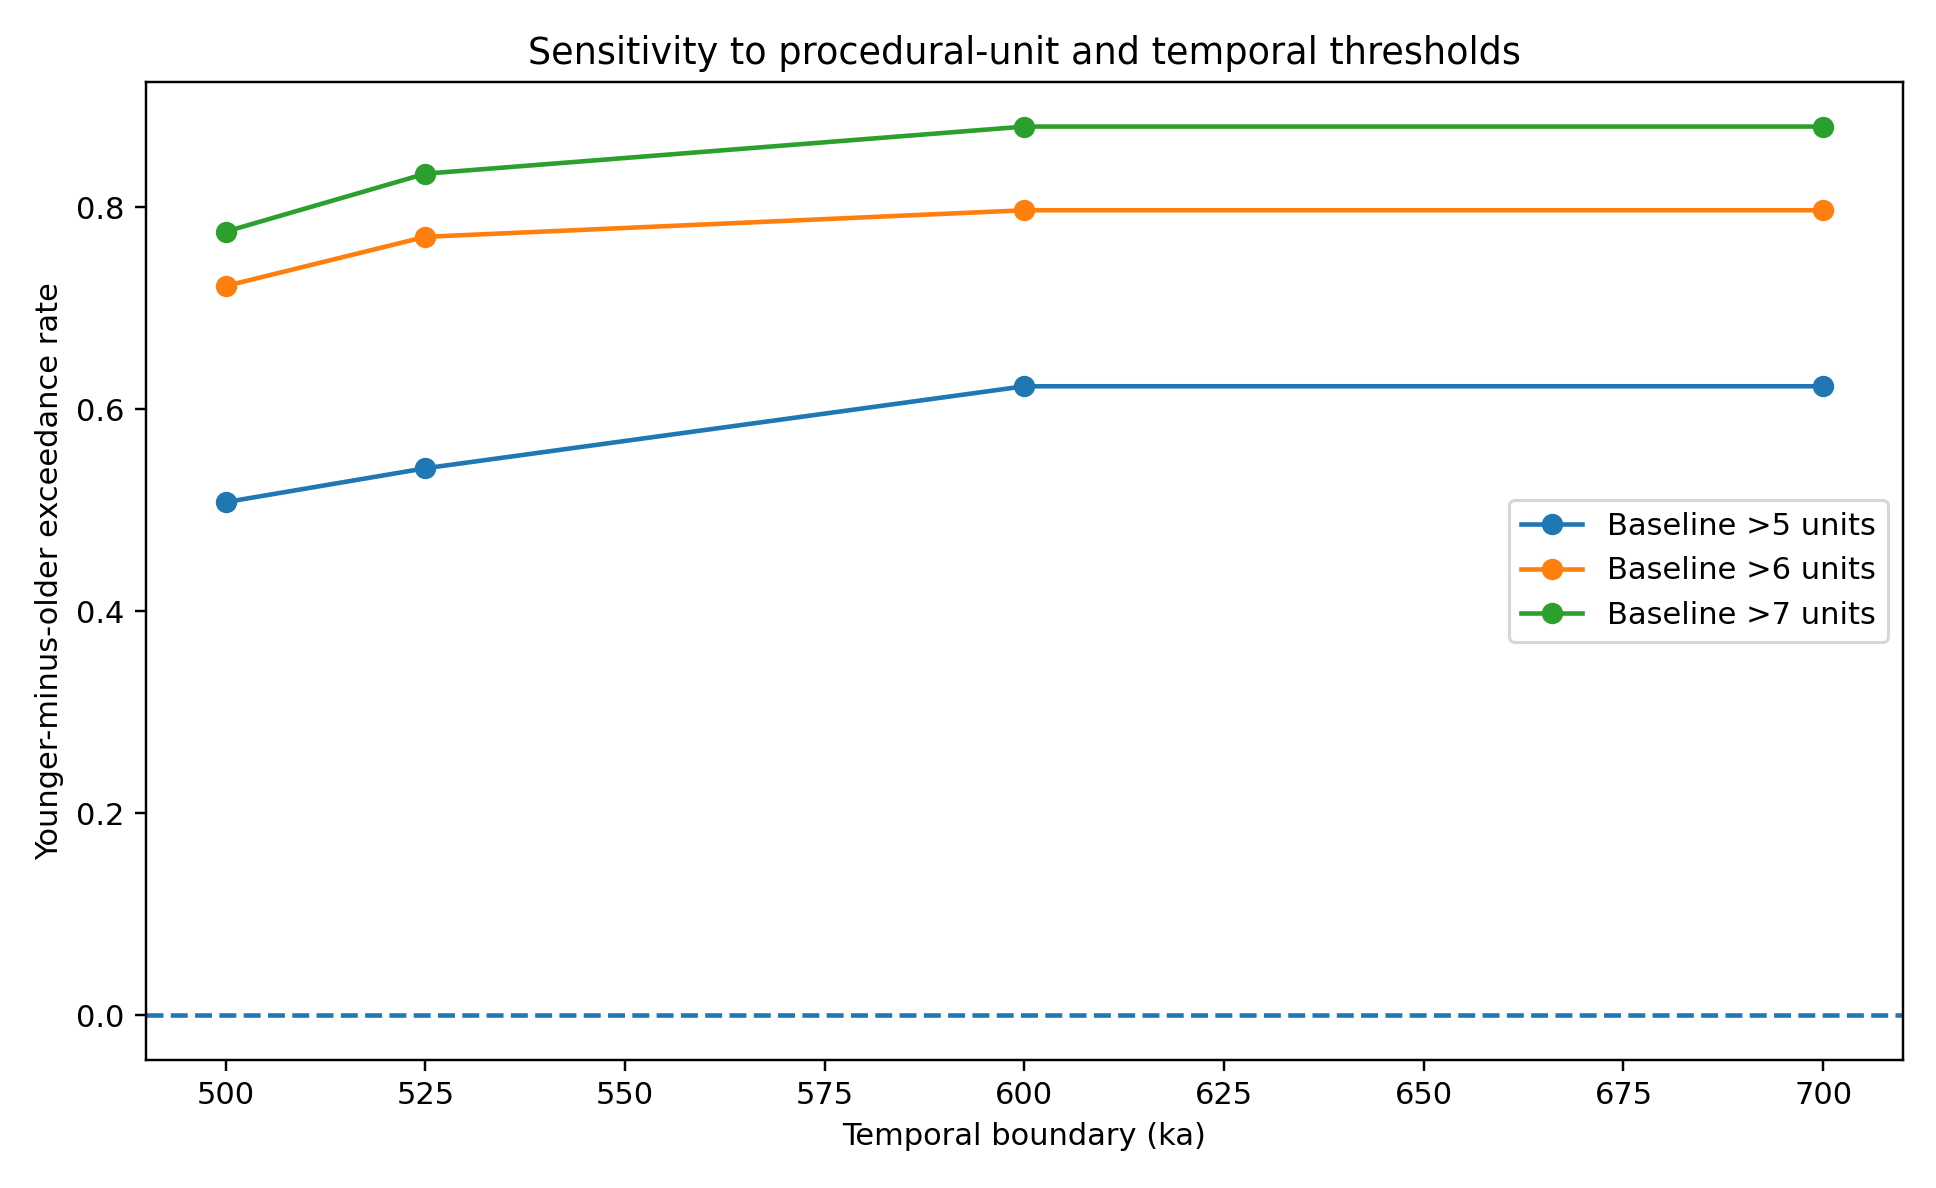
\includegraphics[width=6.1in,height=3.74318in]{figS4.png}
\caption{Plot compares older and younger exceedance rates under
different baselines and temporal boundaries.}
\end{figure}

Figure S4. Sensitivity to procedural baselines and fixed temporal
boundaries.

Table S4. Sensitivity to procedural baseline and temporal boundary.

\begin{longtable}[]{@{}
  >{\raggedright\arraybackslash}p{(\columnwidth - 8\tabcolsep) * \real{0.1948}}
  >{\raggedright\arraybackslash}p{(\columnwidth - 8\tabcolsep) * \real{0.1948}}
  >{\raggedright\arraybackslash}p{(\columnwidth - 8\tabcolsep) * \real{0.1948}}
  >{\raggedright\arraybackslash}p{(\columnwidth - 8\tabcolsep) * \real{0.1948}}
  >{\raggedright\arraybackslash}p{(\columnwidth - 8\tabcolsep) * \real{0.1948}}@{}}
\toprule\noalign{}
\begin{minipage}[b]{\linewidth}\raggedright
Baseline
\end{minipage} & \begin{minipage}[b]{\linewidth}\raggedright
Boundary (ka)
\end{minipage} & \begin{minipage}[b]{\linewidth}\raggedright
Older rate
\end{minipage} & \begin{minipage}[b]{\linewidth}\raggedright
Younger rate
\end{minipage} & \begin{minipage}[b]{\linewidth}\raggedright
Fisher p
\end{minipage} \\
\midrule\noalign{}
\endhead
\bottomrule\noalign{}
\endlastfoot
5 & 500 & 0.471 & 0.979 & 7.67e-06 \\
5 & 525 & 0.438 & 0.979 & 3.68e-06 \\
5 & 600 & 0.357 & 0.980 & 6.67e-07 \\
5 & 700 & 0.357 & 0.980 & 6.67e-07 \\
6 & 500 & 0.235 & 0.957 & 1.63e-08 \\
6 & 525 & 0.188 & 0.958 & 4.00e-09 \\
6 & 600 & 0.143 & 0.940 & 1.13e-08 \\
6 & 700 & 0.143 & 0.940 & 1.13e-08 \\
7 & 500 & 0.118 & 0.894 & 1.08e-08 \\
7 & 525 & 0.062 & 0.896 & 1.41e-09 \\
7 & 600 & 0.000 & 0.880 & 8.10e-10 \\
7 & 700 & 0.000 & 0.880 & 8.10e-10 \\
\end{longtable}

\section{S4. Network-realization
uncertainty}\label{s4.-network-realization-uncertainty}

For stochastic topologies, twenty graphs were independently generated
within every contact stratum, and each graph was paired with eight agent
seeds. Because the graphs differ across contact strata, the bootstrap
resamples graphs independently within each stratum before calculating
pooled p50. It does not construct artificial graph-specific trajectories
across contact levels. Figure S5 shows the pooled curves, and Table S5
reports network-metric associations.

\begin{figure}
\centering
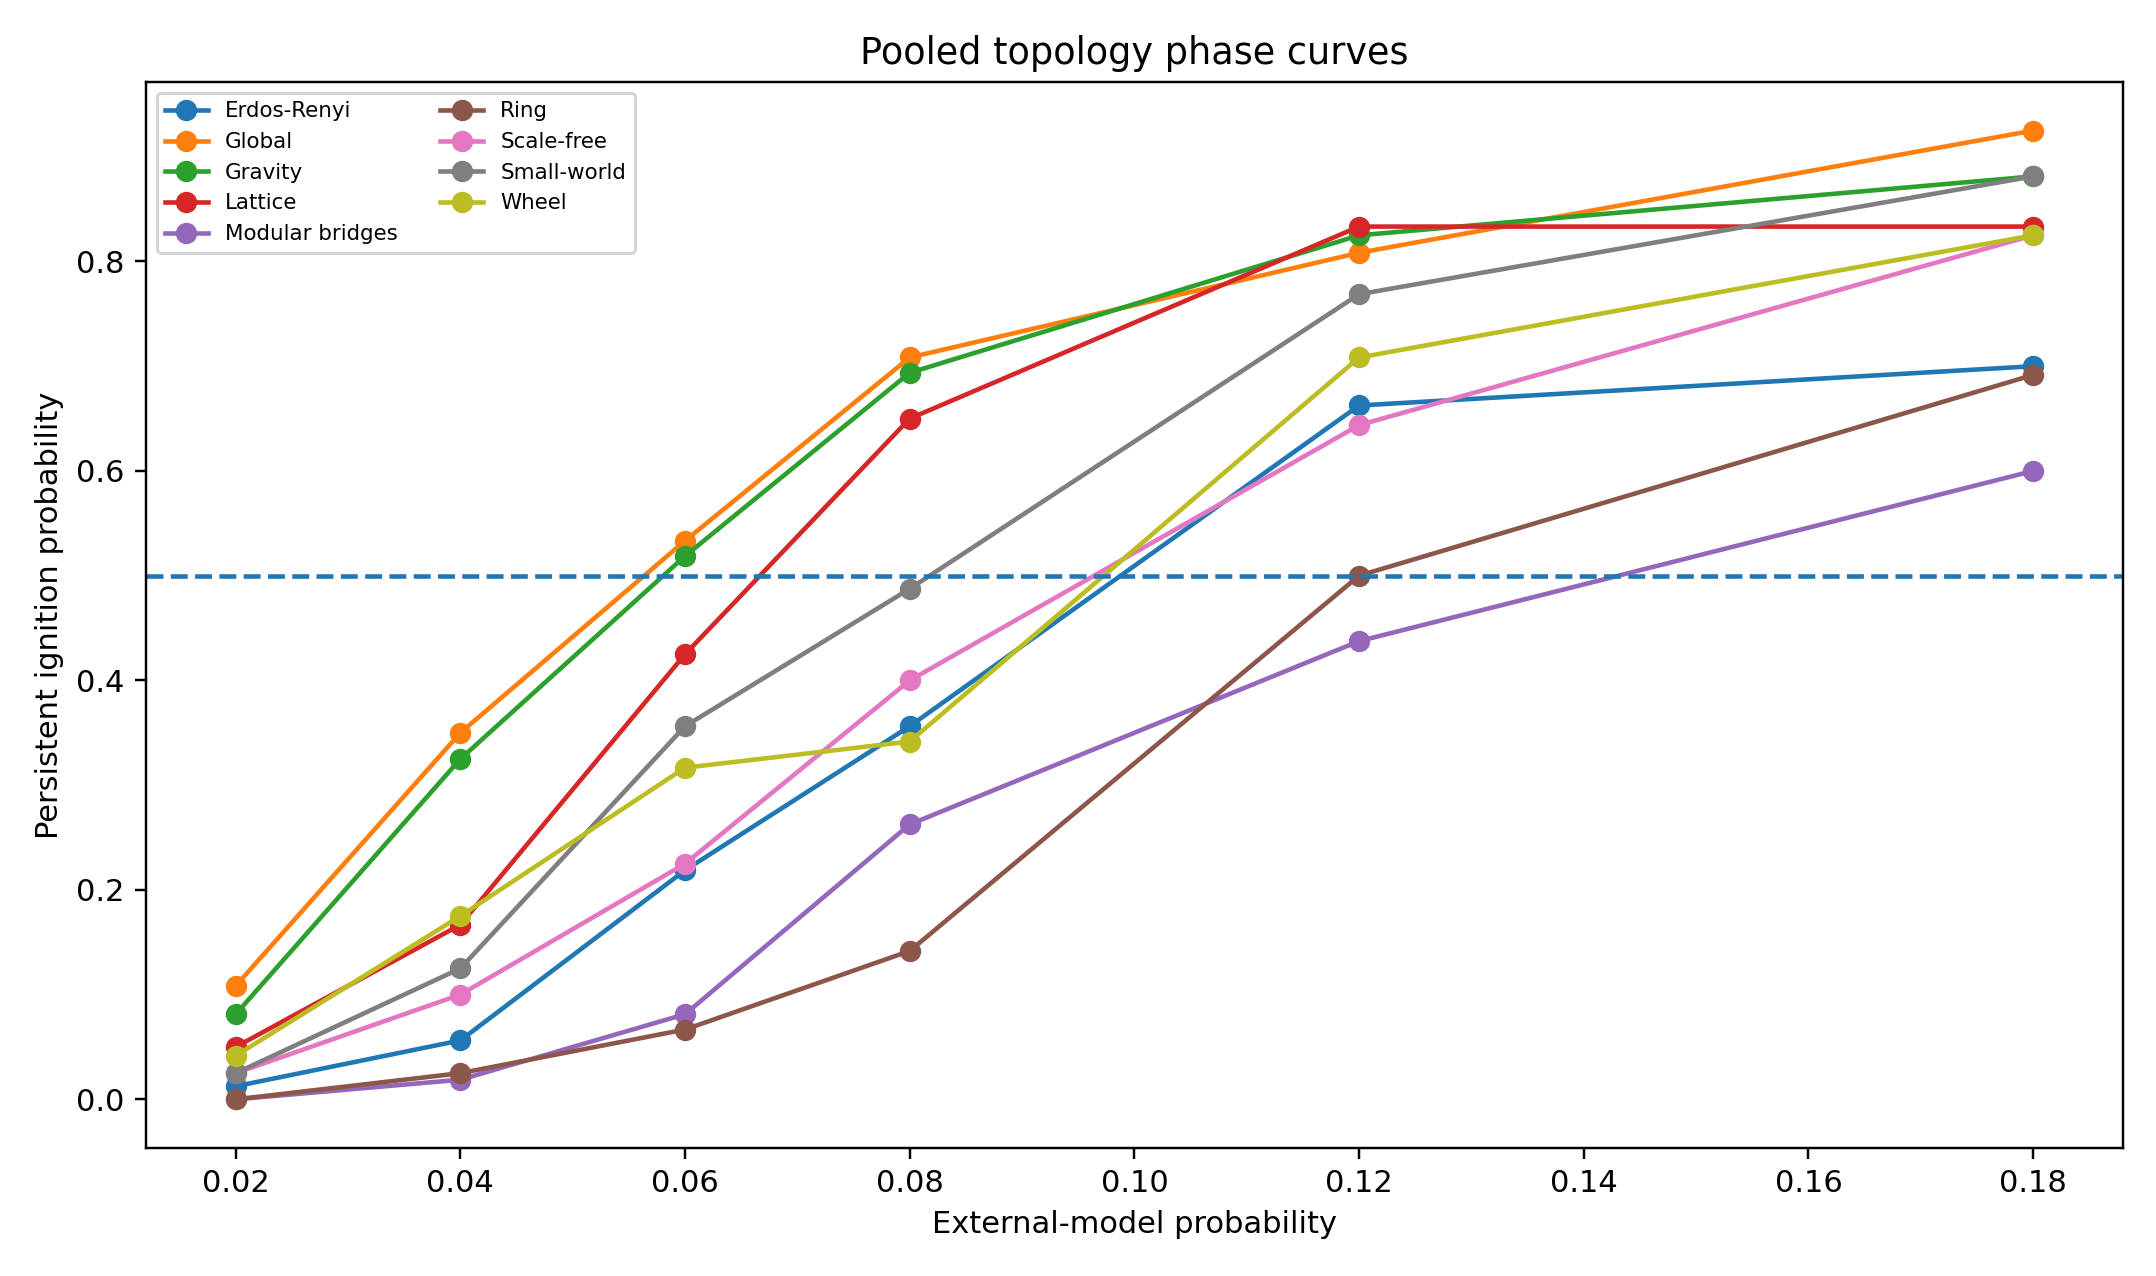
\includegraphics[width=6.35in,height=3.75816in]{figS5.png}
\caption{Nine curves show persistent ignition probability as external
model probability increases.}
\end{figure}

Figure S5. Pooled ignition curves for nine network topologies.

Table S5. Associations between network metrics and contact-adjusted
ignition.

\begin{longtable}[]{@{}
  >{\raggedright\arraybackslash}p{(\columnwidth - 4\tabcolsep) * \real{0.3243}}
  >{\raggedright\arraybackslash}p{(\columnwidth - 4\tabcolsep) * \real{0.3243}}
  >{\raggedright\arraybackslash}p{(\columnwidth - 4\tabcolsep) * \real{0.3243}}@{}}
\toprule\noalign{}
\begin{minipage}[b]{\linewidth}\raggedright
Network metric
\end{minipage} & \begin{minipage}[b]{\linewidth}\raggedright
Spearman rho with contact-adjusted ignition
\end{minipage} & \begin{minipage}[b]{\linewidth}\raggedright
p
\end{minipage} \\
\midrule\noalign{}
\endhead
\bottomrule\noalign{}
\endlastfoot
density & 0.571 & 2.78e-53 \\
clustering & 0.315 & 2.59e-15 \\
mean\_shortest\_path & -0.515 & 7.30e-42 \\
degree\_cv & -0.407 & 2.54e-25 \\
modularity & -0.467 & 9.08e-34 \\
\end{longtable}

\section{S5. Population-architecture
robustness}\label{s5.-population-architecture-robustness}

Table S6 lists the exploratory scaling configurations. Figures S6-S8
separate fixed-total, group-count and group-size effects.

Table S6. Population-architecture robustness ensembles and estimated
thresholds.

\begin{longtable}[]{@{}
  >{\raggedright\arraybackslash}p{(\columnwidth - 10\tabcolsep) * \real{0.2250}}
  >{\raggedright\arraybackslash}p{(\columnwidth - 10\tabcolsep) * \real{0.1500}}
  >{\raggedright\arraybackslash}p{(\columnwidth - 10\tabcolsep) * \real{0.1500}}
  >{\raggedright\arraybackslash}p{(\columnwidth - 10\tabcolsep) * \real{0.1500}}
  >{\raggedright\arraybackslash}p{(\columnwidth - 10\tabcolsep) * \real{0.1500}}
  >{\raggedright\arraybackslash}p{(\columnwidth - 10\tabcolsep) * \real{0.1500}}@{}}
\toprule\noalign{}
\begin{minipage}[b]{\linewidth}\raggedright
Design
\end{minipage} & \begin{minipage}[b]{\linewidth}\raggedright
Groups
\end{minipage} & \begin{minipage}[b]{\linewidth}\raggedright
Group size
\end{minipage} & \begin{minipage}[b]{\linewidth}\raggedright
N
\end{minipage} & \begin{minipage}[b]{\linewidth}\raggedright
p50
\end{minipage} & \begin{minipage}[b]{\linewidth}\raggedright
Status
\end{minipage} \\
\midrule\noalign{}
\endhead
\bottomrule\noalign{}
\endlastfoot
fixed\_group\_20 & 4 & 20 & 80 & & \textgreater0.12 \\
fixed\_group\_20 & 8 & 20 & 160 & 0.067 & estimated \\
fixed\_group\_20 & 16 & 20 & 320 & 0.040 & estimated \\
fixed\_group\_20 & 32 & 20 & 640 & 0.050 & estimated \\
fixed\_group\_20 & 64 & 20 & 1280 & 0.037 & estimated \\
fixed\_groups\_16 & 16 & 10 & 160 & 0.093 & estimated \\
fixed\_groups\_16 & 16 & 20 & 320 & 0.043 & estimated \\
fixed\_groups\_16 & 16 & 40 & 640 & & \textless0.03 \\
fixed\_groups\_16 & 16 & 80 & 1280 & & \textless0.03 \\
fixed\_total\_320 & 4 & 80 & 320 & & \textgreater0.12 \\
fixed\_total\_320 & 8 & 40 & 320 & 0.063 & estimated \\
fixed\_total\_320 & 16 & 20 & 320 & 0.040 & estimated \\
fixed\_total\_320 & 32 & 10 & 320 & 0.070 & estimated \\
\end{longtable}

\begin{figure}
\centering
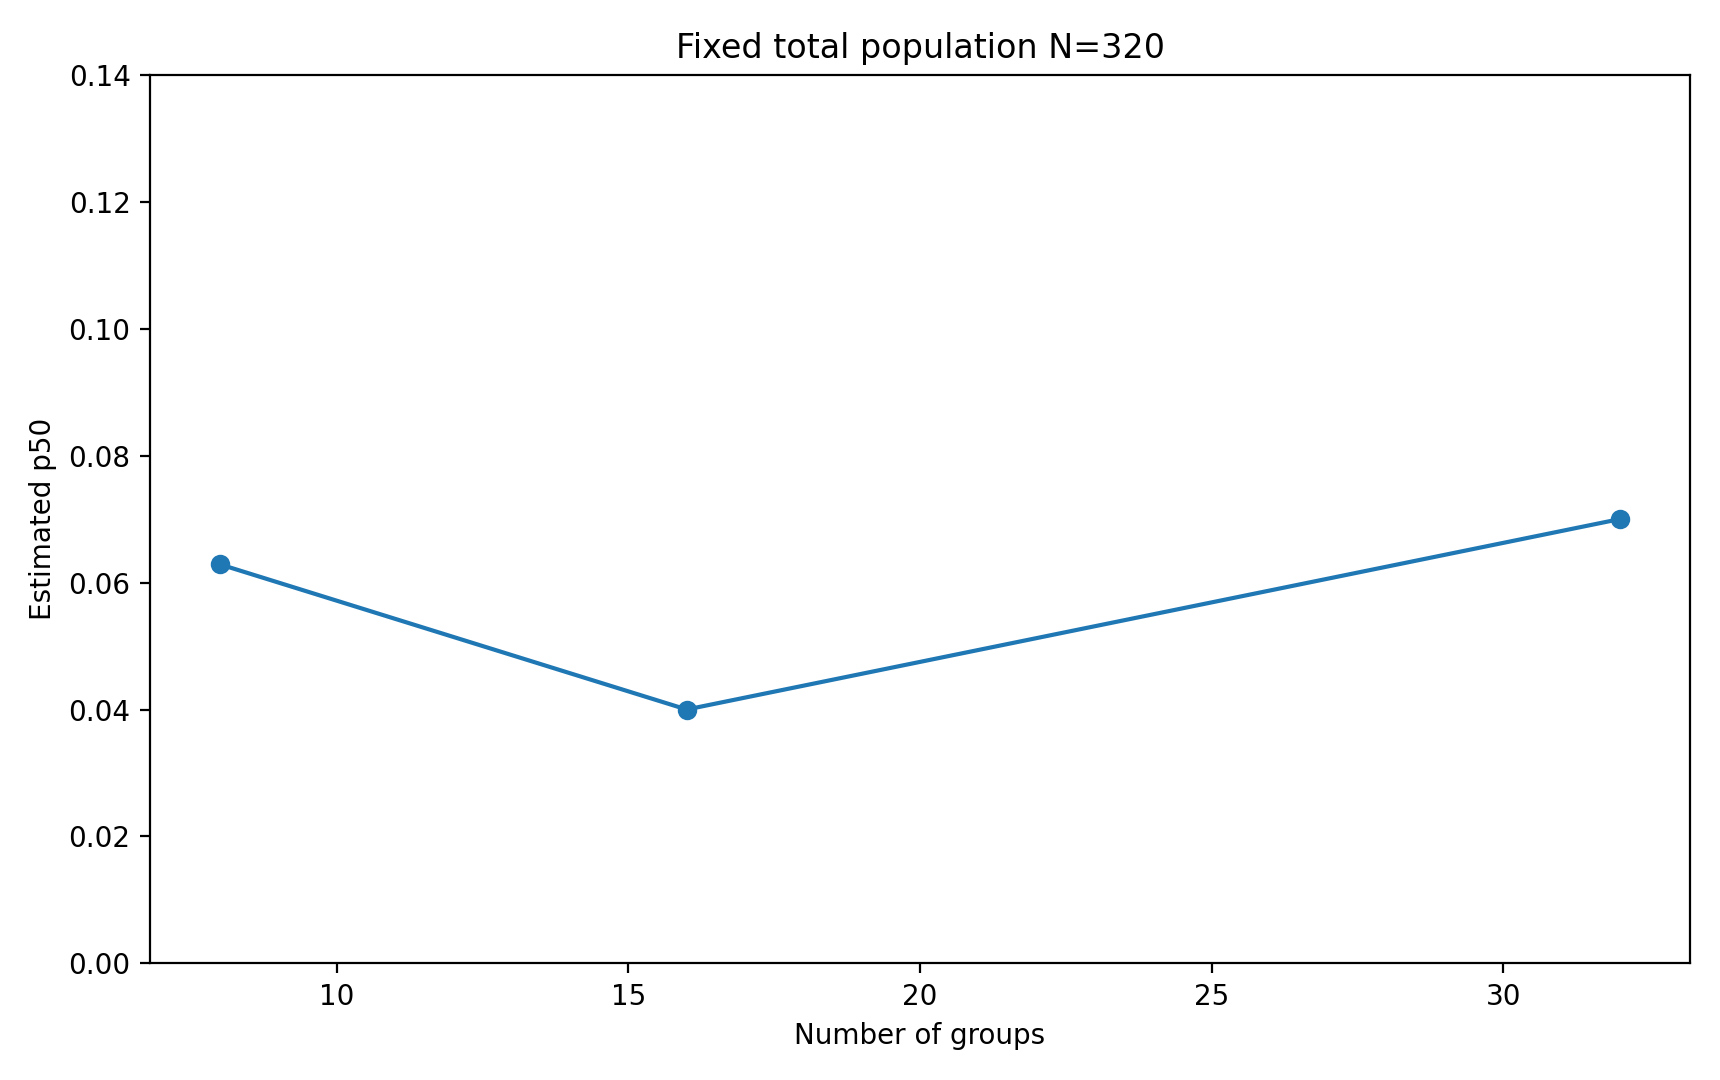
\includegraphics[width=5.8in,height=3.64186in]{figS6.png}
\caption{Line plot of estimated threshold for group partitions with
total population 320.}
\end{figure}

Figure S6. Architecture at fixed total population.

\begin{figure}
\centering
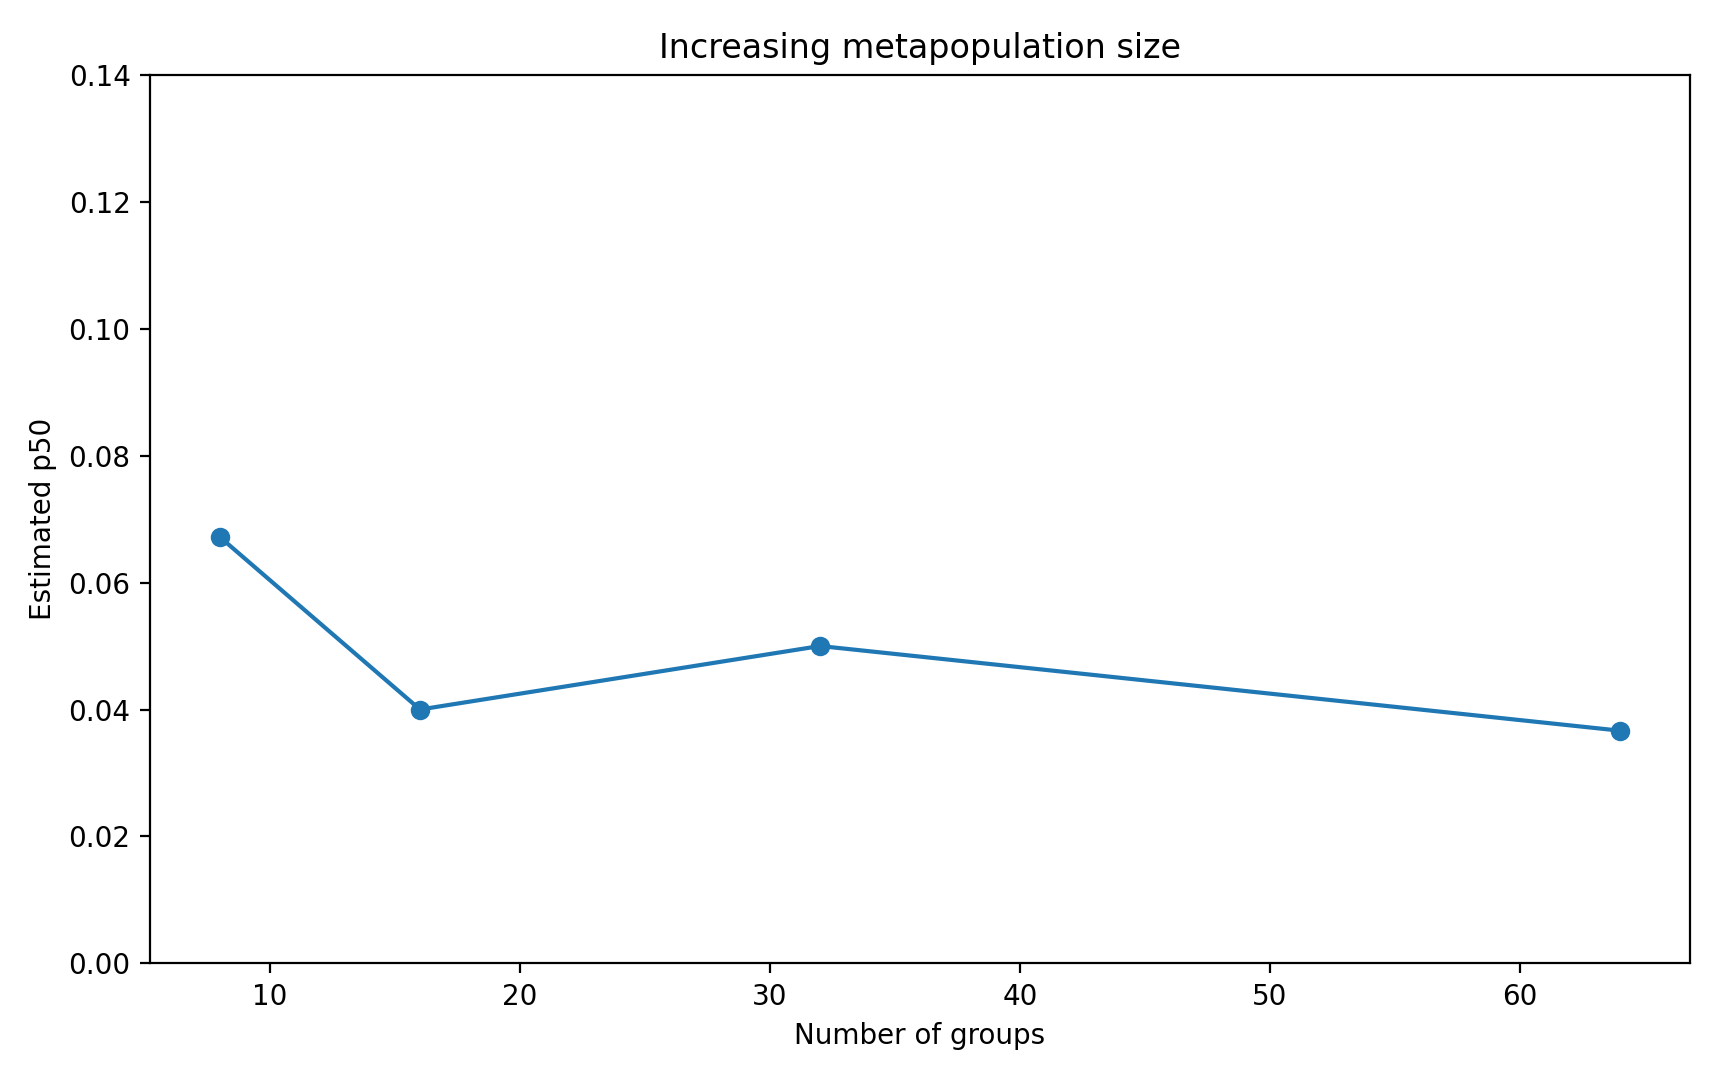
\includegraphics[width=5.8in,height=3.64186in]{figS7.png}
\caption{Line plot of estimated threshold versus number of groups.}
\end{figure}

Figure S7. Robustness to group count with 20 agents per group.

\begin{figure}
\centering
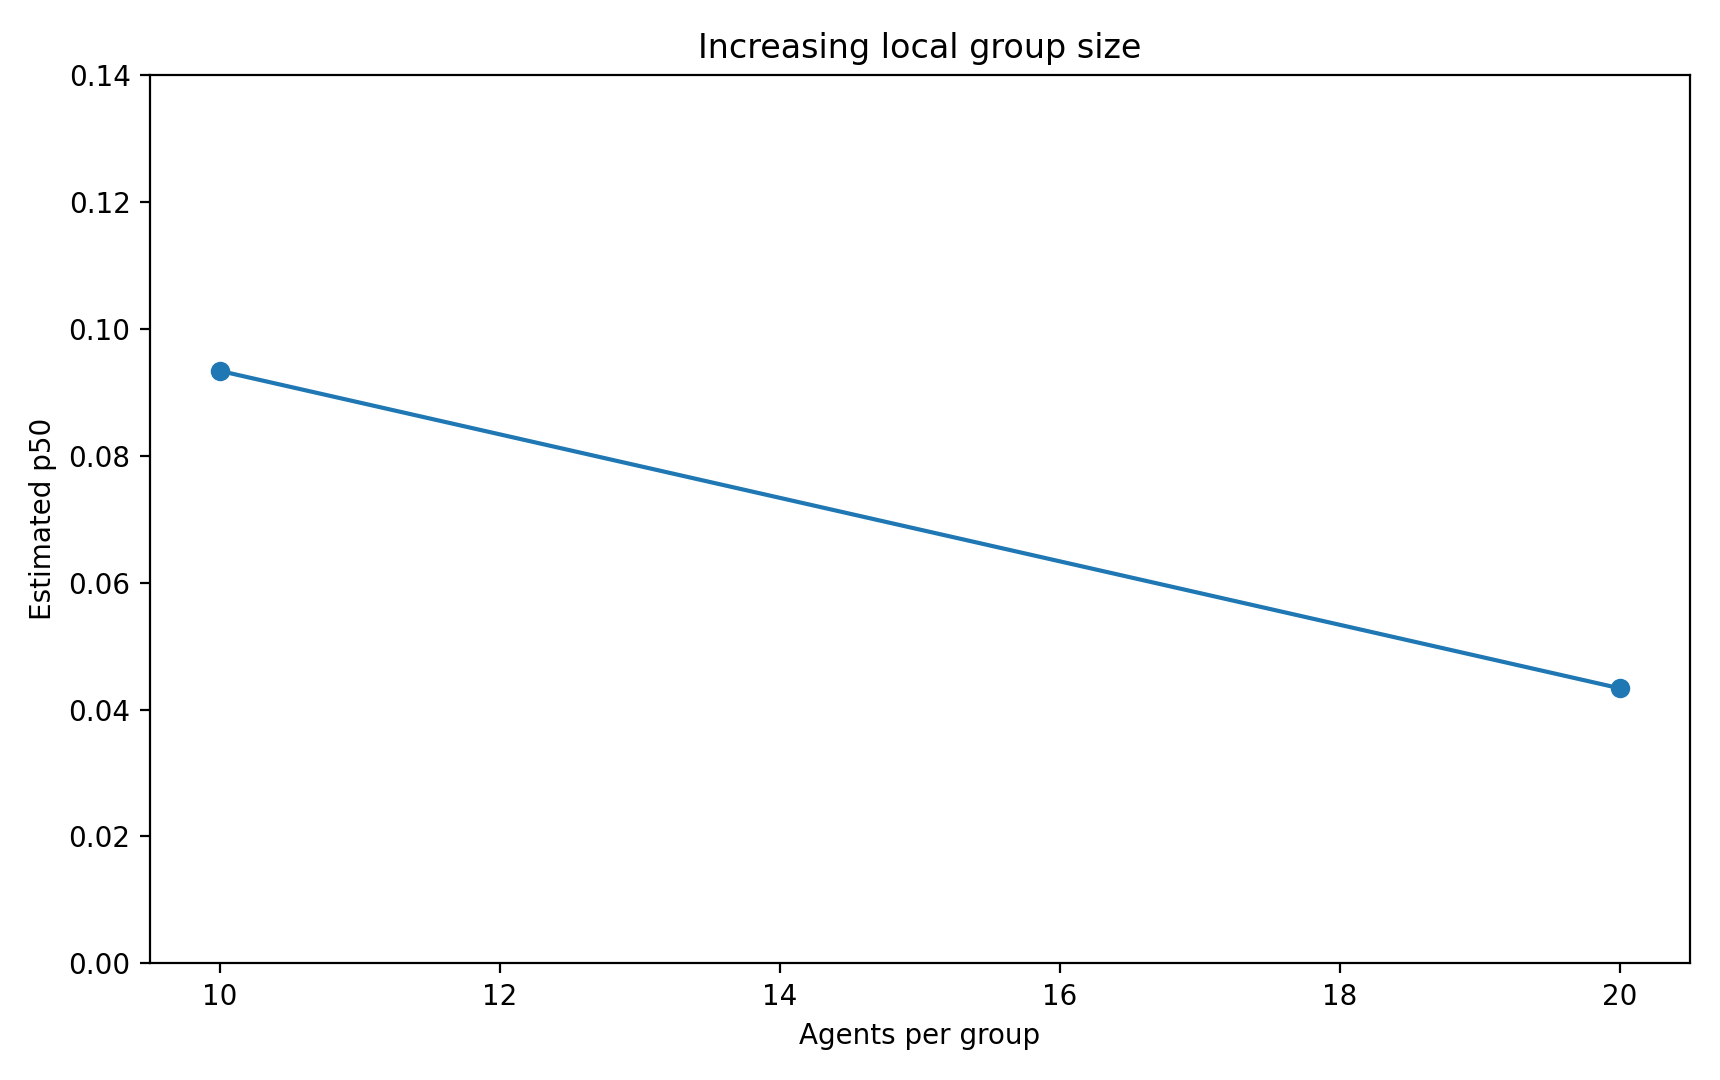
\includegraphics[width=5.8in,height=3.64186in]{figS8.png}
\caption{Line plot of estimated threshold versus agents per group.}
\end{figure}

Figure S8. Robustness to local group size with 16 groups.

\section{S6. Cosmological derivation and
scenarios}\label{s6.-cosmological-derivation-and-scenarios}

Assume successful cultural-ignition events across eligible complex
biospheres form a Poisson process. The mean eligibility exposure
$\bar{E}=\mathbb{E}[E\mid\mathrm{complex\ life}]$ is not estimated from
the archaeological or agent-based data. It is an explicit scenario parameter
defined as the mean eligible duration conditional on a rocky HZ planet already
having reached complex animal-grade life. The separate factor
$f_{\rm complex}$ accounts for the fraction of HZ planets that reach that
state, preventing double counting. The fiducial calculation uses
$\bar{E}=4$ Gyr, and the repository also evaluates 1 and 10 Gyr. All bounds
scale exactly as $1/\bar{E}$. The local ABM probability multiplies, rather
than replaces, the opportunity rate. The firstness probability is conditional
on these assumptions and does not incorporate SETI survey selection,
settlement, detectability or civilisation survival. Table S7 gives the
fiducial filter constraints, Table S8 shows exposure sensitivity, and Figure
S9 shows how contact-dependent $P_{\rm ignite}$ changes the conditional
probability of no earlier successful event.

Table S7. Conditional Great-Filter bounds across Galactic planet-count
scenarios.

\begin{longtable}[]{@{}
  >{\raggedright\arraybackslash}p{(\columnwidth - 4\tabcolsep) * \real{0.3243}}
  >{\raggedright\arraybackslash}p{(\columnwidth - 4\tabcolsep) * \real{0.3243}}
  >{\raggedright\arraybackslash}p{(\columnwidth - 4\tabcolsep) * \real{0.3243}}@{}}
\toprule\noalign{}
\begin{minipage}[b]{\linewidth}\raggedright
NHZ
\end{minipage} & \begin{minipage}[b]{\linewidth}\raggedright
Criterion
\end{minipage} & \begin{minipage}[b]{\linewidth}\raggedright
Maximum $f_{\rm complex}\times r_{\rm opp}$ (Gyr$^{-1}$)
\end{minipage} \\
\midrule\noalign{}
\endhead
\bottomrule\noalign{}
\endlastfoot
1e+08 & 50\% first & 3.466e-09 \\
1e+08 & 95\% first & 2.565e-10 \\
1e+08 & Expected prior \textless1 & 5.000e-09 \\
1e+09 & 50\% first & 3.466e-10 \\
1e+09 & 95\% first & 2.565e-11 \\
1e+09 & Expected prior \textless1 & 5.000e-10 \\
1e+10 & 50\% first & 3.466e-11 \\
1e+10 & 95\% first & 2.565e-12 \\
1e+10 & Expected prior \textless1 & 5.000e-11 \\
\end{longtable}

Table S8. Sensitivity of the 50\% firstness bound to mean eligible exposure
for $N_{\rm HZ}=10^{10}$ and $P_{\rm ignite}=0.5$.

\begin{longtable}[]{@{}lll@{}}
\toprule
$\bar{E}$ (Gyr) & Maximum $f_{\rm complex}r_{\rm opp}$ (Gyr$^{-1}$) & Relative to fiducial \\
\midrule
\endhead
1 & 1.386e-10 & 4.0$\times$ \\
4 & 3.466e-11 & 1.0$\times$ \\
10 & 1.386e-11 & 0.4$\times$ \\
\bottomrule
\end{longtable}

\begin{figure}
\centering
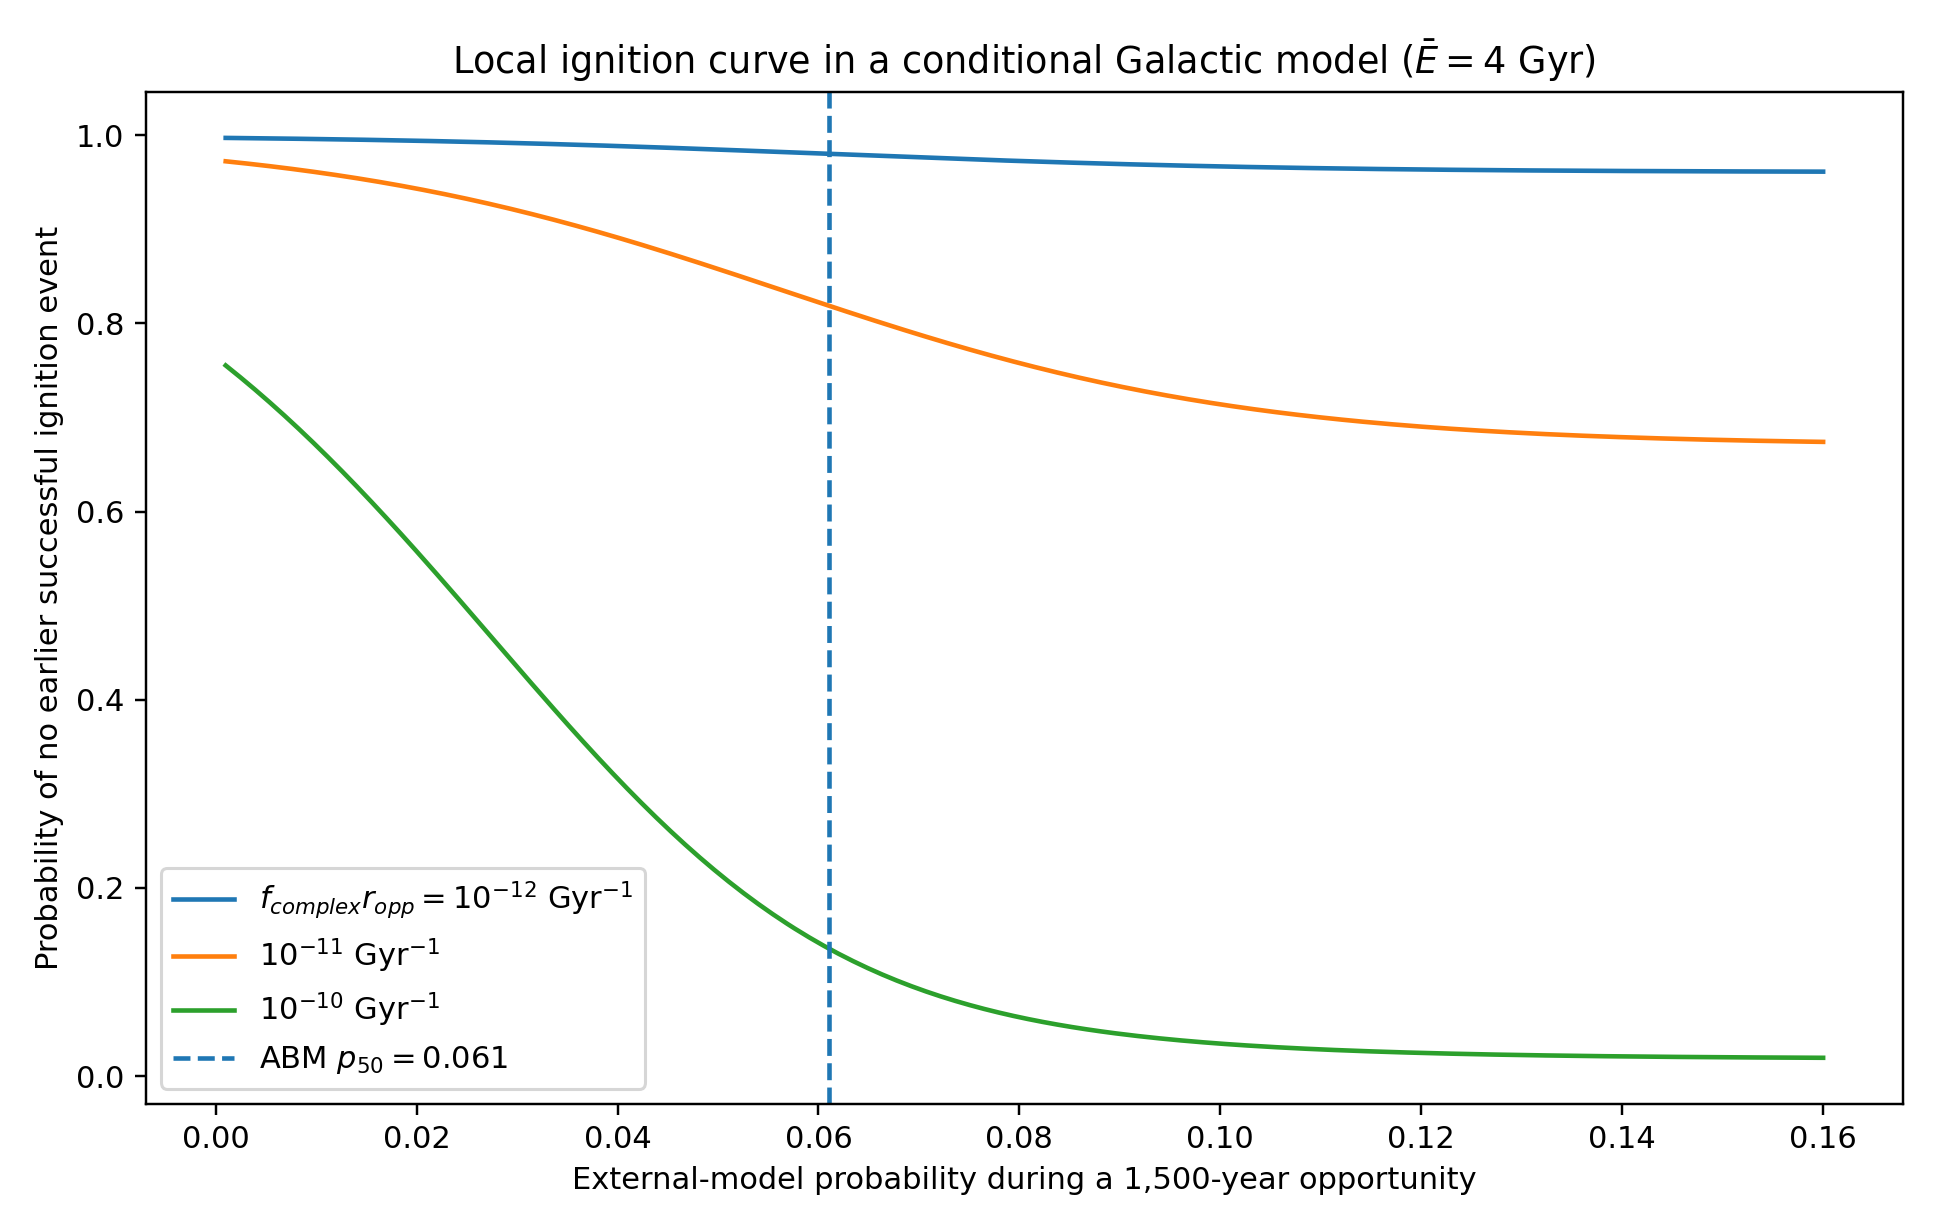
\includegraphics[width=6.15in,height=3.91364in]{figS9.png}
\caption{Conditional probability of no earlier successful ignition event as
external cultural contact changes the local ABM ignition probability. Curves
show three assumed products $f_{\rm complex}r_{\rm opp}$ for
$N_{\rm HZ}=10^{10}$ and $\bar{E}=4$ Gyr.}
\end{figure}

Figure S9. Conditional firstness constraints as contact changes Pignite.

\section{S7. Reproducibility
architecture}\label{s7.-reproducibility-architecture}

The package separates exact reproduction of published summaries from
computationally expensive stochastic regeneration. The preprocessing script
\texttt{prepare\_archaeological\_data.py} rebuilds the 64-row analysis table
from the bundled Windows-1252 source CSV by applying the documented
archaeological and single-chain filters, summing the 33 procedural indicators,
and calculating age midpoints. Frozen ensemble CSV files are the publication
records. The script reproduce\_published\_analyses.py rebuilds the derived
archaeological table and then regenerates archaeological, ablation, topology,
sensitivity, scaling and cosmological summaries and figures.
Stable-seed runners are provided for fresh simulations. The scaling
publication runner uses exactly eight replicates per point, matching the
frozen scaling ensemble; the previous mismatched 20/15 runner has been
removed from the publication package.

\section{S8. Supplementary
references}\label{s8.-supplementary-references}

Barabási, A.-L. and Albert, R. (1999). Emergence of scaling in random
networks. Science 286, 509-512.
https://doi.org/10.1126/science.286.5439.509.

Behroozi, P. and Peeples, M.S. (2015). On the history and future of
cosmic planet formation. Monthly Notices of the Royal Astronomical
Society 454, 1811-1817. https://doi.org/10.1093/mnras/stv1817.

Bryson, S., Kunimoto, M., Kopparapu, R.K. et al.~(2021). The occurrence
of rocky habitable-zone planets around solar-like stars from Kepler
data. Astronomical Journal 161, 36.
https://doi.org/10.3847/1538-3881/abc418.

Cantor, M., Chimento, M., Smeele, S.Q. et al.~(2021). Social network
architecture and the tempo of cumulative cultural evolution. Proceedings
of the Royal Society B 288, 20203107.
https://doi.org/10.1098/rspb.2020.3107.

Carroll-Nellenback, J., Frank, A., Wright, J. and Scharf, C. (2019). The
Fermi paradox and the Aurora effect: exo-civilization settlement,
expansion and steady states. Astronomical Journal 158, 117.
https://doi.org/10.3847/1538-3881/ab31a3.

Deffner, D., Fedorova, N., Andrews, J. and McElreath, R. (2024).
Bridging theory and data: a computational workflow for cultural
evolution. Proceedings of the National Academy of Sciences USA 121,
e2322887121. https://doi.org/10.1073/pnas.2322887121.

Derex, M. and Boyd, R. (2015). The foundations of the human cultural
niche. Nature Communications 6, 8398.
https://doi.org/10.1038/ncomms9398.

Derex, M., Perreault, C. and Boyd, R. (2018). Divide and conquer:
intermediate levels of population fragmentation maximize cultural
accumulation. Philosophical Transactions of the Royal Society B 373,
20170062. https://doi.org/10.1098/rstb.2017.0062.

Erdős, P. and Rényi, A. (1959). On random graphs I. Publicationes
Mathematicae Debrecen 6, 290-297.
https://doi.org/10.5486/PMD.1959.6.3-4.12.

Fay, N., De Kleine, N., Walker, B. and Caldwell, C.A. (2019). Increasing
population size can inhibit cumulative cultural evolution. Proceedings
of the National Academy of Sciences USA 116, 6726-6731.
https://doi.org/10.1073/pnas.1811413116.

Gunasekaram, C. et al.~(2024). Population connectivity shapes the
distribution and complexity of chimpanzee cumulative culture. Science
386, 920-925. https://doi.org/10.1126/science.adk3381.

Hagberg, A.A., Schult, D.A. and Swart, P.J. (2008). Exploring network
structure, dynamics, and function using NetworkX. In Proceedings of the
7th Python in Science Conference, pp.~11-15.

Harris, C.R., Millman, K.J., van der Walt, S.J. et al.~(2020). Array
programming with NumPy. Nature 585, 357-362.
https://doi.org/10.1038/s41586-020-2649-2.

Holland, P.W., Laskey, K.B. and Leinhardt, S. (1983). Stochastic
blockmodels: first steps. Social Networks 5, 109-137.
https://doi.org/10.1016/0378-8733(83)90021-7.

Kandel, A.W., Sommer, C., Kanaeva, Z., Bolus, M. et al.~(2023). The
ROCEEH Out of Africa Database (ROAD): a large-scale research database
for human evolutionary studies. PLOS ONE 18, e0289513.
https://doi.org/10.1371/journal.pone.0289513.

Kipping, D. (2020). An objective Bayesian analysis of
life\textquotesingle s early start and our late arrival. Proceedings of
the National Academy of Sciences USA 117, 11995-12003.
https://doi.org/10.1073/pnas.1921655117.

Kirby, S. and Tamariz, M. (2022). Cumulative cultural evolution,
population structure and the origin of combinatoriality in human
language. Philosophical Transactions of the Royal Society B 377,
20200319. https://doi.org/10.1098/rstb.2020.0319.

Kolodny, O., Creanza, N. and Feldman, M.W. (2015). Evolution in leaps:
the punctuated accumulation and loss of cultural innovations.
Proceedings of the National Academy of Sciences USA 112, E6762-E6769.
https://doi.org/10.1073/pnas.1520492112.

Loeb, A., Batista, R.A. and Sloan, D. (2016). Relative likelihood for
life as a function of cosmic time. Journal of Cosmology and
Astroparticle Physics 2016(08), 040.
https://doi.org/10.1088/1475-7516/2016/08/040.

Mesoudi, A. and Thornton, A. (2018). What is cumulative cultural
evolution? Proceedings of the Royal Society B 285, 20180712.
https://doi.org/10.1098/rspb.2018.0712.

Mills, D.B., Macalady, J.L., Frank, A. and Wright, J.T. (2025). A
reassessment of the hard-steps model for the evolution of intelligent
life. Science Advances 11, eads5698.
https://doi.org/10.1126/sciadv.ads5698.

Montrey, M. and Shultz, T.R. (2020). The evolution of high-fidelity
social learning. Proceedings of the Royal Society B 287, 20200090.
https://doi.org/10.1098/rspb.2020.0090.

Morgan, T.J.H., Uomini, N.T., Rendell, L.E. et al.~(2015). Experimental
evidence for the co-evolution of hominin tool-making, teaching and
language. Nature Communications 6, 6029.
https://doi.org/10.1038/ncomms7029.

Muthukrishna, M., Doebeli, M., Chudek, M. and Henrich, J. (2018). The
cultural brain hypothesis: how culture drives brain expansion, sociality
and life history. PLOS Computational Biology 14, e1006504.
https://doi.org/10.1371/journal.pcbi.1006504.

Paige, J. and Perreault, C. (2023). A dataset describing the
manufacturing of stone tools over 3 million years. Journal of Open
Archaeology Data 11, 12. https://doi.org/10.5334/joad.114.

Paige, J. and Perreault, C. (2024). 3.3 million years of stone tool
complexity suggests cumulative culture began during the Middle
Pleistocene. Proceedings of the National Academy of Sciences USA 121,
e2319175121. https://doi.org/10.1073/pnas.2319175121.

Pearce, E. and Moutsiou, T. (2014). Using obsidian transfer distances to
explore social network maintenance in late Pleistocene hunter-gatherers.
Journal of Anthropological Archaeology 36, 12-20.
https://doi.org/10.1016/j.jaa.2014.07.002.

Prokopenko, M., Ay, N., Breviario, A. et al.~(2026). Algorithmic
bottlenecks in evolution: genetic code, symbolic language, and the Great
Filter hypothesis. arXiv:2605.04498.
https://doi.org/10.48550/arXiv.2605.04498.

Schleicher, D.R.G. and Bovino, S. (2023). The Fermi paradox: impact of
astrophysical processes and dynamical evolution. International Journal
of Astrobiology 22, 1-14. https://doi.org/10.1017/S147355042200026X.

Shkurko, A.V. (2024). The social science perspective on the Fermi
paradox. International Journal of Astrobiology 23, e13.
https://doi.org/10.1017/S1473550424000089.

van Leeuwen, E.J.C., DeTroy, S.E., Haun, D.B.M., Call, J. et al.~(2024).
Chimpanzees use social information to acquire a skill they fail to
innovate. Nature Human Behaviour 8, 891-902.
https://doi.org/10.1038/s41562-024-01836-5.

Virtanen, P., Gommers, R., Oliphant, T.E. et al.~(2020). SciPy 1.0:
fundamental algorithms for scientific computing in Python. Nature
Methods 17, 261-272. https://doi.org/10.1038/s41592-019-0686-2.

Walker, B. and Fay, N. (2026). Identifying the necessary conditions for
large populations to enhance cumulative culture. Scientific Reports 16,
10090. https://doi.org/10.1038/s41598-026-40973-x.

Watts, D.J. and Strogatz, S.H. (1998). Collective dynamics of
small-world networks. Nature 393, 440-442.
https://doi.org/10.1038/30918.

Winters, J. and Charbonneau, M. (2026). Modelling the emergence of
open-ended cultural evolution. Philosophical Transactions of the Royal
Society B 381, 20250255. https://doi.org/10.1098/rstb.2025.0255.

Wright, J.T., Kanodia, S. and Lubar, E.G. (2018). How much SETI has been
done? Finding needles in the n-dimensional cosmic haystack. Astronomical
Journal 156, 260. https://doi.org/10.3847/1538-3881/aae099.

\end{document}
